\documentclass[11pt]{article}
\usepackage{amsmath, amssymb, amscd, amsthm, amsfonts}
\usepackage{graphicx}
\usepackage{hyperref}
\usepackage{acronym}
\usepackage{listings}
\usepackage[margin=2cm]{geometry}
\usepackage{endnotes}

% for pseudocode
\usepackage{algorithm}
\usepackage[noend]{algpseudocode}

% change language to german
\usepackage[utf8]{inputenc}
\usepackage[T1]{fontenc}
\usepackage[ngerman]{babel}
\usepackage{hyphenat}
% ---------

% for code style
\usepackage{xcolor}

\definecolor{codegreen}{rgb}{0,0.6,0}
\definecolor{codegray}{rgb}{0.5,0.5,0.5}
\definecolor{codepurple}{rgb}{0.58,0,0.82}
\definecolor{backcolour}{rgb}{0.95,0.95,0.92}

\lstdefinestyle{mystyle}{
    backgroundcolor=\color{backcolour},   
    commentstyle=\color{codegreen},
    keywordstyle=\color{magenta},
    numberstyle=\tiny\color{codegray},
    stringstyle=\color{codepurple},
    basicstyle=\ttfamily\footnotesize,
    breakatwhitespace=false,         
    breaklines=true,                 
    captionpos=b,                    
    keepspaces=true,                 
    numbers=left,                    
    numbersep=5pt,                  
    showspaces=false,                
    showstringspaces=false,
    showtabs=false,                  
    tabsize=2
}

\lstset{style=mystyle}
% ----------------------

\usepackage{glossaries}

\oddsidemargin 0pt
\evensidemargin 0pt
\marginparwidth 40pt
\marginparsep 10pt
\topmargin -20pt
\headsep 10pt
\textheight 8.7in
\textwidth 6.65in
\linespread{1}

% for centering the title page
\usepackage{titling}
\renewcommand\maketitlehooka{\null\mbox{}\vfill}
\renewcommand\maketitlehookd{\vfill\null}

% usesul macros
\newcommand{\lstin}[1]{\lstinline[language=C]{#1}}
\newcommand{\cpl}{\textbf{C}$\;$}

% for footnotes
\renewcommand{\notesname}{Fußnoten}
\let\footnote=\endnote

% ------- glossary -------
% to build the glossary when changed run the build make_glossaries.cmd file first
\makeglossaries

% TODO: sources for definitions
\newglossaryentry{bm}
{
  name=Benchmark,
  description={Test für die Zeitkomplexität und Speicherkomplextät von Software},
}

\newglossaryentry{opl}
{
  name=OpenGL,
  description={TODO},
}
% ------- acronyms -------
\newacronym{rbt}{RBT}{Red Black Tree}

% ------- glossary -------

\title{\textbf{Multimedia-Projektarbeit}}
\author{Yannik Höll \& Christoph Paul Pooch \& Marie Luise Clemenz \& Viktoryia Talaknianik}
\date{\today}

\begin{document}

\begin{titlingpage}
    \maketitle
\end{titlingpage}
\pagebreak

\tableofcontents
\pagebreak

\glsaddall
\printglossary 
\pagebreak

\section{Einleitung} 
% Einleitungssätze
Eins der wohl bekanntesten Computerspiele ist Tetris. Denkbar einfach, allerdings stecken hinter
dem recht trivialen Spiel doch im Nachhinein gesehen sehr viele aufwendige Funktionen.

% Ziel der Arbeit
In der folgenden Dokumentation wird erläutert, wie die Implementierung des bekannten Spiels in \gls{opl} 
umgesetzt wurde und welche Herausforderungen gelöst werden mussten.


\section{Theoretische Grundlagen}
% Bibliotheken
% Sprache

\section{Codedokumentation}

\subsection{Grobstruktur}

\begin{lstlisting}[language=C]
enum GameState {
    PAUSE,      // Game paused while in menu
    PLAYING,    // Main gamestate where the pieces are moving
    GAME_OVER   // After losing the game, this gamestate is reached
};

struct GameData {
    enum GameState gameState;

    int* current_piece;             // current piece, no fixed size
    int* next_piece;                // save the next piece for the display
    int* arena;                     // width: 10, height: 20 -> 200 uints

    int position_x;                 // position of the current piece inside the arena
    int position_y;

    bool fast_drop;                 // flag that determines whether the pieces move slow or fast downwards
                                    // enabled when player presses the down button

    uint32_t score;
    uint32_t level;                 // level for piece velocity
    uint32_t cleared_lines;

    int* piece_count;               // saves the number of times the piece have shown up

    double accumulated_time;        // current playing time

    bool is_defeat;                 // detemins wheter the player has lost

    uint32_t seed;                  // for playing a certain game
};

\end{lstlisting}

\begin{figure}[h]
  \centering
  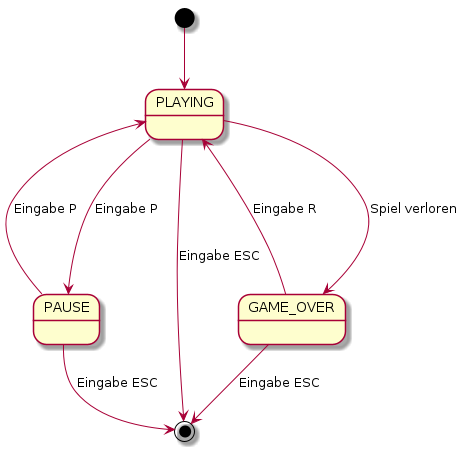
\includegraphics[width=0.5\textwidth]{../state.png}
  \caption{Zustandsdiagramm}
\end{figure}

\subsection{Implementierung}

\section{Projektdokumentation}

\subsection{Tools \& Entwicklungsumgebung}
Github-umgebung
Oben GL

\subsection{Arbeitsaufteilung}

\section{Benutzerhandbuch}

\pagebreak
\bibliographystyle{alpha}
\bibliography{references} % see references.bib for bibliography management

\end{document}

% for citation:
% \cite{aad} for simple citation
% \cite[S. 20]{aad} for citation with page number(s)

% for acronyms and glossary ref:
% https://en.wikibooks.org/wiki/LaTeX/Glossary
% \gls{acro-name}

% Listings Example:
% \begin{lstlisting}[language=C]
%         #include <stdio.h>
%        
%         int main(void)
%         {
%                 printf("Hello, World\n");
%                 return EXIT_SUCCESS;
%         }
% \end{lstlisting}

% TODO: 
% Definitions
% Reference for Stackoverflow recursion depth in defs and traversal
% Pictures for tree and for tree array represantation